\documentclass{article}

\usepackage{html}
\usepackage{graphicx}

\begin{document}

This page contains links to writings about topics such as technology, video games, and philosophy.

\tableofchildlinks*

% Gentoo Portage tree local sync
% Internet Security and the Technocracy
% X.509
% Facebook targeting children

% Ancient Apparition Bowling
\section{2017-07-17 Ancient Apparition Bowling}
This is a silly metagame that I came up with for a DotA2 custom game.  It may not be possible to beat, but I've yet to try all strategies.

\subsection*{Origin}
Mercilessly slaughtering bots using weird combinations of cheats in DotA2 is an easy way to blow off a little steam after a difficult match.  One day I decided to go "bowling" with Ancient Apparition; I'd cheat to maximum level, 6-slot, enable wtf mode, and snipe the bots from base with his ultimate.
This is loads of fun, until the creeps start pushing towers, at which point the bots also take advantage of wtf mode and begin spamming fortify, leading to a frustrating stalemate.  The workaround for this is to disable wtfmode and instead use the \texttt{-refresh} cheat, which, although it does reset fortify cooldowns, can be used in conjunction with a Refresher Orb to blast the bots with two ultimates while giving them only one fortify.

The result is a semi-functional slaughtering of bots, although having to constantly open the command prompt to paste and submit the \texttt{-refresh} command gets annoying after a while; sadly, there doesn't seem to be a way to disable the bots' fortify spam.  After a little bit of this, I noticed that the cooldown of the metaphorical bowling ball and the travel time were not that far apart, leading me to wonder if I could play this game successfully without having to spam cheat commands (and reset the fortify cooldown) all game long.  Thus "Ancient Apparition Bowling" was born.

\subsection*{Rules}
These are the rules of the game, and though they may not be comprehensive, you should be able to understand the jist of them.  First, stay in fountain for the duration of the match.  Second, use cheats to give yourself max level (\texttt{-lvlup 25}), 6-slots (\texttt{-item <name>}), and vision (\texttt{-allvision}).  Third, no backpack, stash, or other item-use shenanegains; stick to your 6 slots. (TODO: pic of fountain)  Fourth, no bots on your team and five bots of highest difficulty on the other team.  That's it!
\begin{figure}
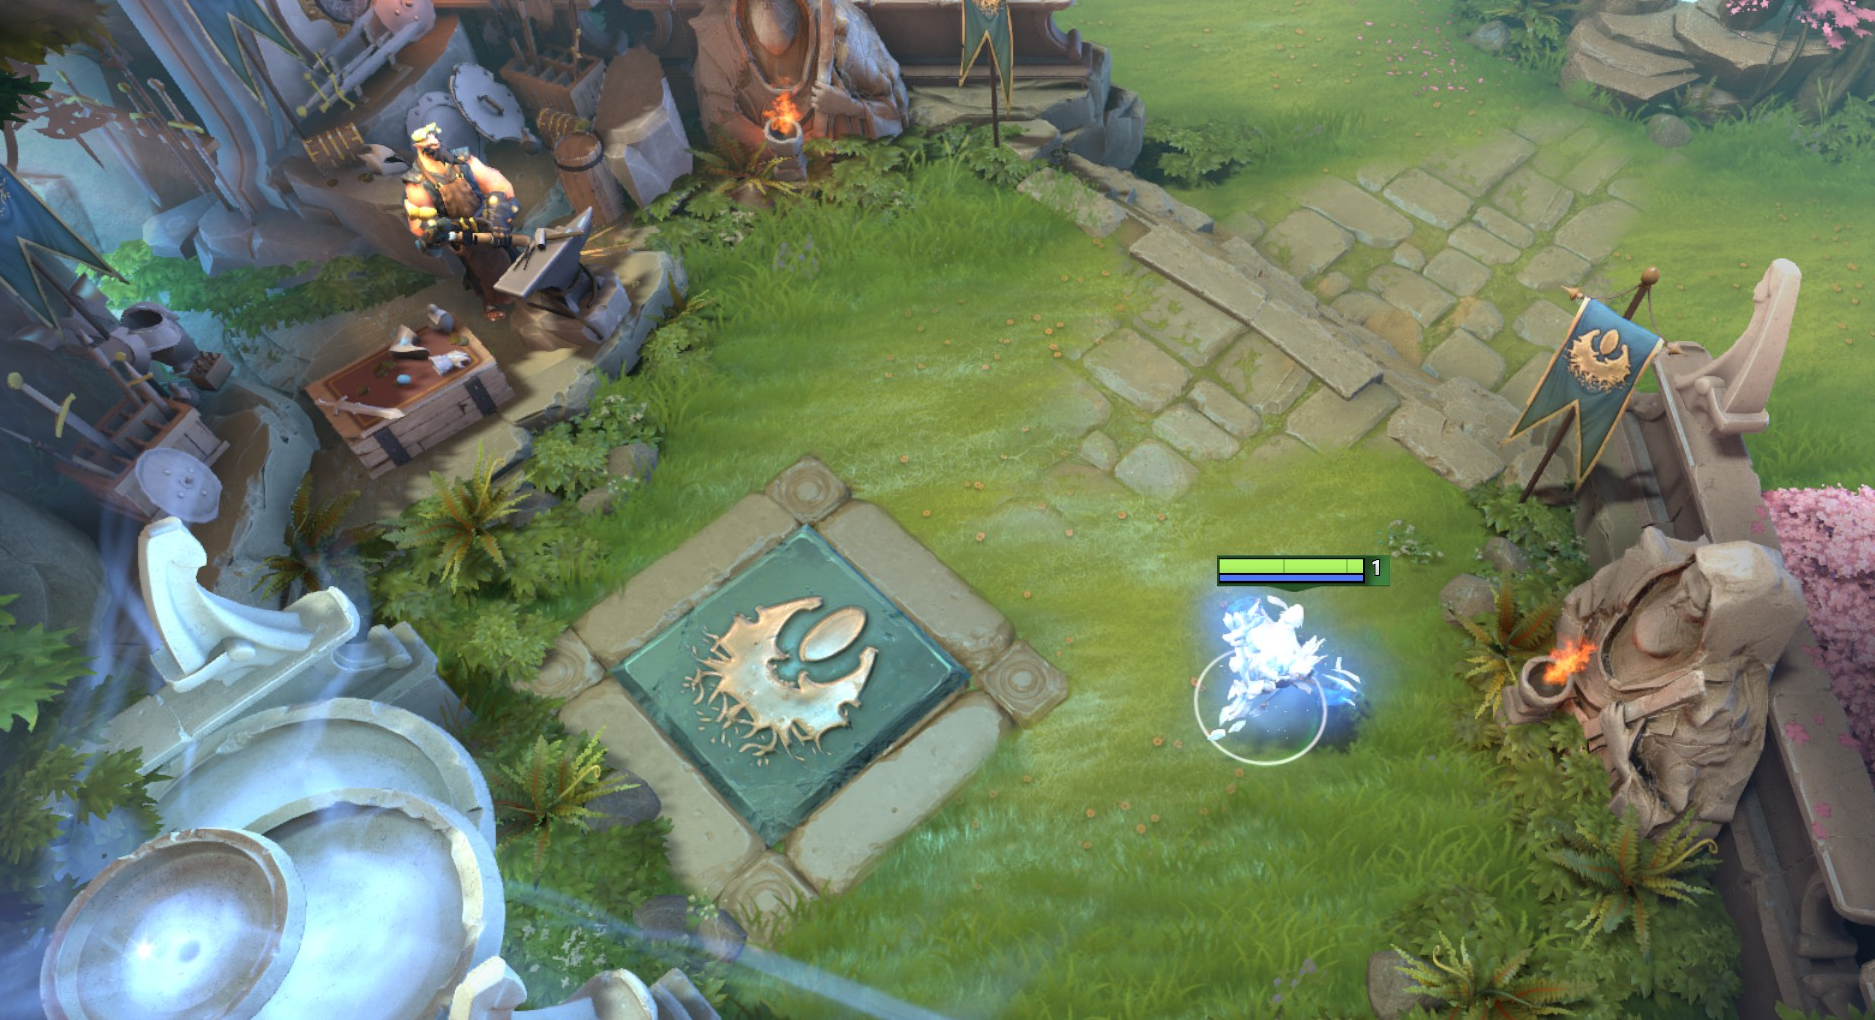
\includegraphics[scale=0.33]{files/blog/2017_07_17_ancient_apparition_bowling/fountain.png}
\caption{Where you will be spending all of your time.}
\end{figure}

Your goal is now to destroy the bots' ancient before the bots level up enough to tank through your ult and push your base.  This is more difficult than it sounds, as the bots are actually rather crafty and level up sooner than you might expect.

\subsection*{Strategy}
My current build involves getting an Aghaim's Scepter, Octarine Core, Refresher Orb, and 3 Aether Lens (TODO: picture of items).  Perhaps you can think up something better.
\begin{figure}
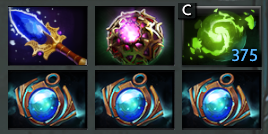
\includegraphics{files/blog/2017_07_17_ancient_apparition_bowling/items.png}
\end{figure}

It is difficult to push all lanes at once, since the bots can quickly respawn at lower levels, and you only have so many ultimates to shoot off.  It would thus seem prudent to choose a particular lane to hammer, but how to do so isn't actually obvious.

The strategy that I tried was to focus the enemy creeps at their spawning point in a side lane.  This can be done by firing consistently at the 18 and 48 second marks towards the front of their 3rd tower. This will obliterate all of the creeps during the early part of the game.  Make sure to adjust your ultimate slightly to the left each time in order to adjust for the micro-delay between your ult going off cooldown and actually launching your ult; you can reset this after a while with a Refresher Orb.
\begin{figure}
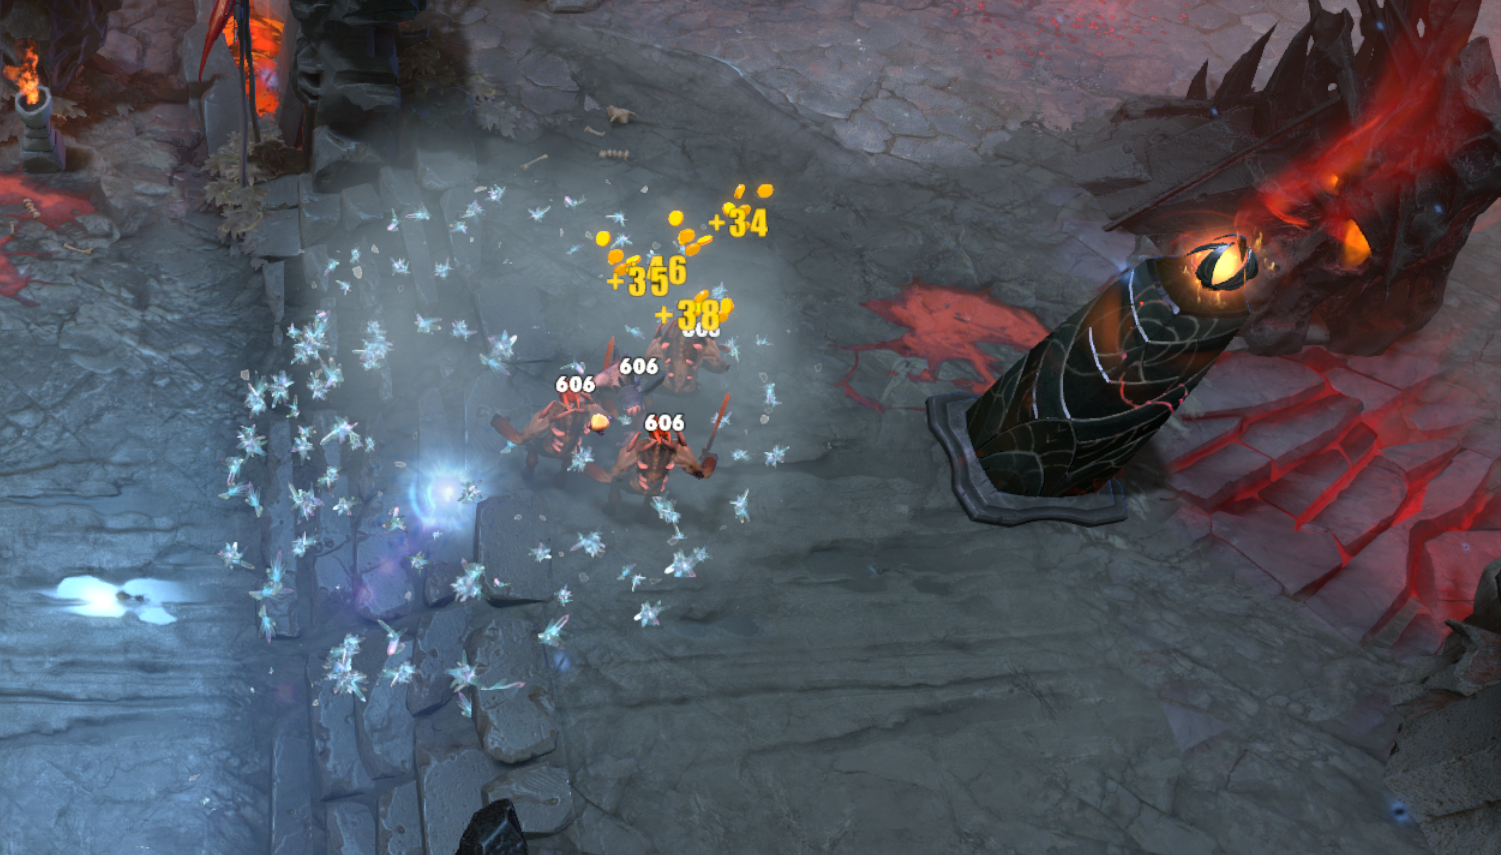
\includegraphics[scale=0.33]{files/blog/2017_07_17_ancient_apparition_bowling/towerhit.png}
\caption{Killing creeps as soon as they spawn.}
\end{figure}

Though this may at first seem like a good way to get the creeps to push the tower, the bots are actually crafty enough to pull the creeps behind the tower, limiting the amount of damage done.  While I was able to eventually push to their barracks, at this point the other bots also helped pull the creeps behind the barracks, and eventually became strong enough to tank the ult and push my base, thus making this a losing strategy.
\begin{figure}
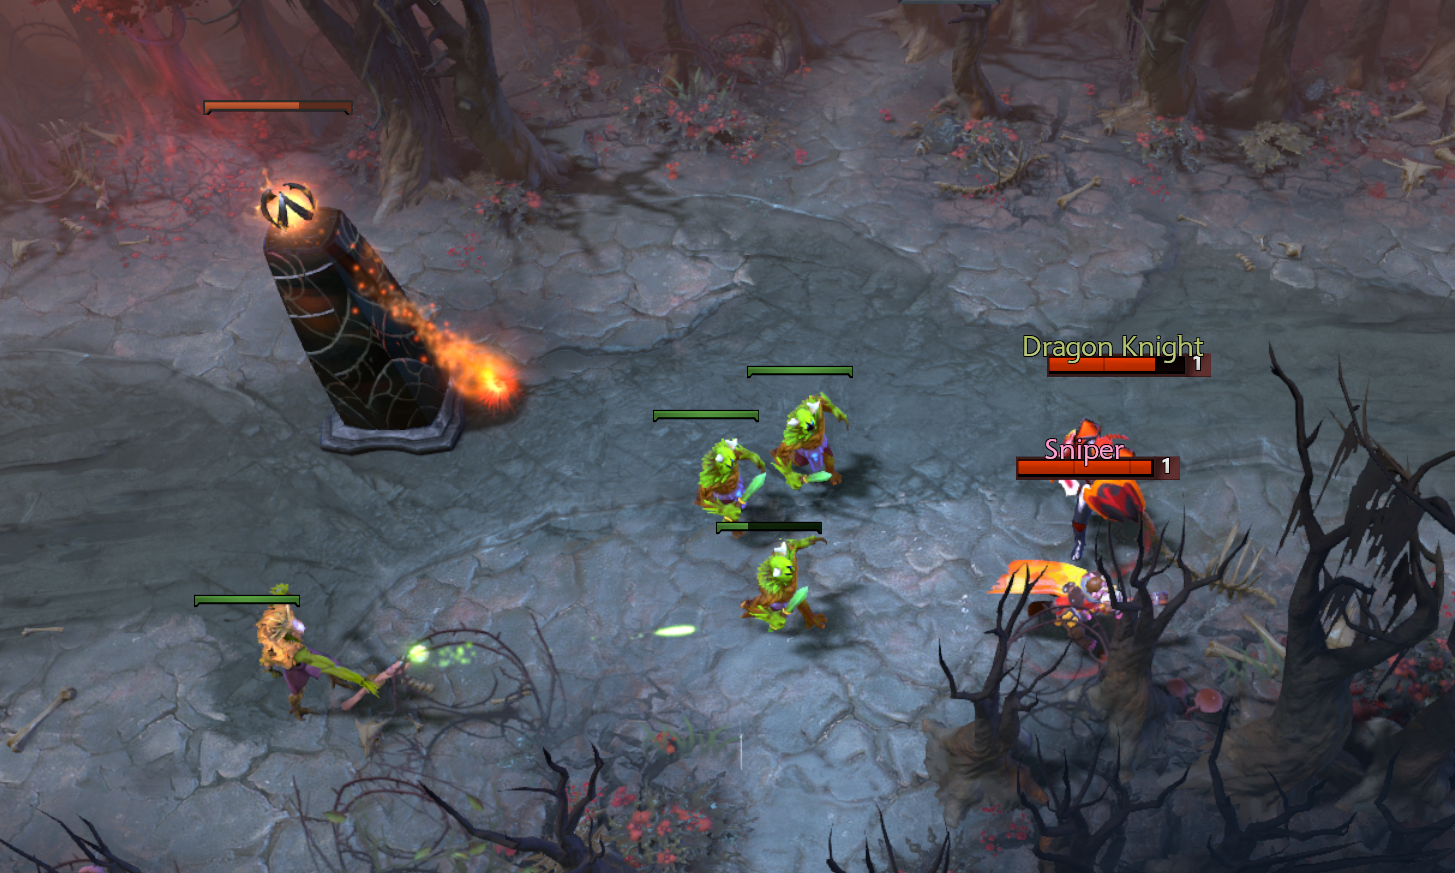
\includegraphics[scale=0.33]{files/blog/2017_07_17_ancient_apparition_bowling/botpull.png}
\caption{Sneaky bots pulling creeps away from the tower.}
\end{figure}

A possible variation would be to try focusing down the bots themselves, but this is tricky as they often move out of the ult's way.  A hybrid combination may involve finding a position where the bots and creeps are likely to align, then aiming to kill the creeps and probably the bots.  It may also be easier to push straight up middle rather than taking out a side lane first, especially as the bots seem found of charging up mid.

I've yet to win at this metagame.  It might not even be plausible.  Try it yourself and see what happens!

\subsection*{Addendum}
Between inventing this game, writing this article, and getting the screenshots, the bot fortify spam in wtf mode seems to have stopped.

\end{document}
